\documentclass[a4paper]{article}
\usepackage{WUST-AAE-NMaO-Report}
\usepackage{natbib}

\usepackage{amsmath}
% \usepackage{amssymb}
% \usepackage[polish,main=english]{babel}
% \usepackage{titlesec}
% \usepackage{vmargin}
% \usepackage{graphicx}
% \graphicspath{{images/}}
% \usepackage{fancyhdr}
% \usepackage{systeme}
% \usepackage{xcolor}
% \usepackage{indentfirst}
% \usepackage{xspace}
% \newcommand{\MATLAB}{\textsc{Matlab}\xspace}
% \usepackage{listings}
% \usepackage{matlab-prettifier}
% \usepackage{hyperref}
% \usepackage{multicol}


% \newcommand{\sectionbreak}{\clearpage}
% \setmarginsrb{3 cm}{2.5 cm}{3 cm}{2.5 cm}{1 cm}{1.5 cm}{1 cm}{1.5 cm}

% Augmented matrix
% \newenvironment{amatrix}[2]{%
  % \left[\begin{array}{@{}*{#1}{c} | c *{#2}{c} @{}}
% }{%
  % \end{array}\right]
% }

% Bold letters in matrices
% \newcommand{\matr}[1]{\mathbf{#1}}

%%%%%%%%%%%%%%%%%%%%%%%%%%%%%%%%%%%%%%%

\title{Numerical Algorithms – Report 1: Direct Methods for Solving Linear Systems}
\author{Sergiusz Warga 230757}
\date{\today}
\reporttutor{dr hab. inż. Rafał Zdunek}

\begin{document}

\maketitle
\tableofcontents
\pagebreak

%%%%%%%%%%%%%%%%%%%%%%%%%%%%%%%%%%%%%%

\section{Problems calculations}
\subsection{Problem 1}%
\label{sec:problem_1}
Find the solution that best approximates the system of inconsistent linear equations:
\begin{tasks}(3)
  \task $\systeme{3x_1-x_2=4,x_1+2x_2=0,2x_1+x_2=1}$
  \task $\systeme{3x_1+x_2+x_3=6,
  2x_1+3x_2-x_3=1,
  2x_1-x_2+x_3=0,
  3x_1-3x_2+3x_3=8}$
  \task $\systeme{x_1+x_2-x_3=5,
  2x_1-x_2+6x_3=1,
  -x_1+4x_2+x_3=0,
  3x_1+2x_2-x_3=6}$
\end{tasks}
%%%%%%%%%%%%%%%%%%%%%%%%%%%%%%%%%%%%%%%%%%%%%%%%%%%%%%%%%%%%%%%%%%%%%%%%%%%%%%%
\subsubsection*{Mathematics}
%%%%%%%%%%%%%%%%%%%%%%%%%%%%%%%%%%%%%%%%%%%%%%%%%%%%%%%%%%%%%%%%%%%%%%%%%%%%%%%
The system of inconsistent linear equations comprises linearly independent equations,
whose number is greater than the number of unknown variables.
Such a system may be expressed in the form:
\begin{equation*}
  \matr{Ax}=\matr{b}, \quad \text{where} \quad
  \matr{A}\in\mathfrak{R}^{m\times{}n}, \quad
  \matr{b}\in\mathfrak{R}^m, \quad
  \matr{x}\in\mathfrak{R}^n, \quad \text{and} \quad m\geq{}n
\end{equation*}
and has no solution. We may attempt to find the best approximate solution to such a
system by solving the minimization problem:
\begin{equation*}
  \min_{\matr{x}}{\left\lVert\matr{b}-\matr{A}\matr{x}\right\rVert}_2
\end{equation*}
For such a system, an associated system of \textit{normal equations} is defined to be:
\begin{equation}
  \matr{A}^T\matr{Ax}=\matr{A}^T\matr{b}
\end{equation}
which is always consistent.
The solution has the form:
\begin{equation}
  \label{eq:normal_approximation}
  \matr{x}=\left(\matr{A}^T\matr{A}\right)^{-1}\matr{A}^T\matr{b}
\end{equation}
%%%%%%%%%%%%%%%%%%%%%%%%%%%%%%%%%%%%%%%%%%%%%%%%%%%%%%%%%%%%%%%%%%%%%%%%%%%%%%%
\subsubsection*{Solution}
%%%%%%%%%%%%%%%%%%%%%%%%%%%%%%%%%%%%%%%%%%%%%%%%%%%%%%%%%%%%%%%%%%%%%%%%%%%%%%%
The solutions to all the systems of linear equations above may be easily approximated
with the \MATLAB{} function implementing~\eqref{eq:normal_approximation}:
\lstinputlisting[style=Matlab-editor]{problems/normal_approximation.m}
Then, the solution may be verified with \lstinline[style=Matlab-editor]{x - A\b}:
\lstinputlisting[style=Matlab-editor]{problems/Problem_1.m}

% \subsection{Problem 2}\label{problem:2}
Solve the following system of linear equations using the Gaussian elimination with pivoting:
\begin{equation*}
    \systeme{x_1+x_2+x_3=1,x_1+x_2+2x_3=2,x_1+2x_2+2x_3=1}
\end{equation*}
Explain why the Gaussian elimination without pivoting does not work.
\subsubsection*{Mathematics}
As was stated at the end of the theoretical introduction to the previous problem, Gaussian Elimination algorithms require the diagonal entry to be different than zero (to not normalize the row dividing by zero). While in manual computations such a division would be noticed, in \MATLAB their result is \texttt{Inf} and algorithm proceeds with replacing subsequent coefficients with this value, resulting in gibberish output. With pivoting this behaviour can be avoided. The basic idea is to find a maximum absolute value in the zeroed column below the pivot and interchange their rows. This is called a partial pivoting. Searching in the whole sub-matrix spanned between pivot and $A_{n,m}$, therefore interchanging not only rows but also columns, is called a complete pivoting.
\subsubsection*{Solution}
\begin{equation*}
\begin{split}
    \begin{amatrix}{1}{1}
        \matr{A} & \matr{b}
    \end{amatrix} = 
    \begin{amatrix}{3}{1}
        1 & 1 & 1 & 1\\
        1 & 1 & 2 & 2\\
        1 & 2 & 2 & 1
    \end{amatrix} \xrightarrow[\substack{R_2-R_1\\R_3-R_1}]{}
    \begin{amatrix}{3}{1}
        1 & 1 & 1 & 1\\
        0 & 0 & 1 & 1\\
        0 & 1 & 1 & 0
    \end{amatrix} \xrightarrow[R_2\leftrightarrow R_3]{}
    \begin{amatrix}{3}{1}
        1 & 1 & 1 & 1\\
        0 & 1 & 1 & 0\\
        0 & 0 & 1 & 1
    \end{amatrix}\rightarrow\\
    \rightarrow
    \systeme{x_1+x_2+x_3=1,x_2+x_3=0,x_3=1}
    \rightarrow
    \systeme{x_1+x_2+x_3=\phantom{-}1,x_2=-1,x_3=\phantom{-}1}
    \rightarrow
    \begin{cases}
    x_1=\phantom{-}1\\
    x_2=-1\\
    x_3=\phantom{-}1
    \end{cases}
\end{split}
\end{equation*}

To verify manual solution the Algorithm~\ref{algorithm:2} was used. As is explained in detail in~\cite[section 3.4.2]{GoluVanl96} it transforms matrix $\matr{P}\matr{A}\matr{U}$ into a form from which lower unit triangular and upper triangular matrices may be extracted, so that:
\begin{align*}
   \matr{P}\matr{A}\matr{U} &= \matr{L}\matr{U} & \matr{A}\matr{x}&=\matr{b}
\end{align*}
therefore
\begin{align*}
    \matr{A}&=\matr{P^T}\matr{L}\matr{U}\matr{Q^T} & \matr{P^T}\matr{L}\matr{U}\matr{Q^T}\matr{x} &= \matr{b}\\
    & & \matr{L}\matr{U}\matr{Q^T}\matr{x} &= \matr{P}\matr{b}
\end{align*}
\lstinputlisting[style=Matlab-editor]{problems/Problem2.m}\\
% \subsection{Problem 3}
Solve the system:
\begin{equation*}
    \systeme{0.0001x_1+x_2=1,x_1+x_2=2}
\end{equation*}
with the Gaussian elimination with and without pivoting at the round-off error limited to 3 significant digits. Compute the condition number of the system matrix.
\subsubsection*{Mathematics}
Not only pivoting helps with $a_{ii}=0$ problem but, by choosing the biggest entry, ensures the stability of the LU factorization. As explained in detail in~~\cite[section 3.3]{GoluVanl96} for the factorization errors to be small, the diagonal entries of $\matr{U}$ matrix has to be small. Please note that in both solutions and condition number computations precision was limited to 3 significant digits.
\subsubsection*{Solution without pivoting}
\begin{equation*}
\begin{split}
    \begin{amatrix}{1}{1}
        \matr{A} & \matr{b}
    \end{amatrix} = 
    \begin{amatrix}{2}{1}
        10^{-4} & 1 & 1\\
        1 & 1 & 2
    \end{amatrix}
    \xrightarrow[\substack{R_2-10^{4}R_1}]{}
    \begin{amatrix}{2}{1}
        10^{-4} & 1 & 1\\
        0 & -10^{4} & -10^{4}
    \end{amatrix}
\end{split}
\end{equation*}
gives us
\begin{equation*}
    \begin{cases}
    x_1=0\\
    x_2=1\\
    \end{cases}
\end{equation*}
which is obviously contradictory to $R_2$.

\subsubsection*{Solution with pivoting}
\begin{equation*}
\begin{split}
    \begin{amatrix}{1}{1}
        \matr{A} & \matr{b}
    \end{amatrix} = 
    \begin{amatrix}{2}{1}
        10^{-4} & 1 & 1\\
        1 & 1 & 2
    \end{amatrix}
    \xrightarrow[R_1\leftrightarrow R_2]{}
    \begin{amatrix}{2}{1}
        1 & 1 & 2 \\
        10^{-4} & 1 & 1
    \end{amatrix}
    \xrightarrow[\substack{R_2-10^{-4}R_1}]{}
    \begin{amatrix}{2}{1}
        1 & 1 & 2 \\
        0 & 1 & 1
    \end{amatrix}
\end{split}
\end{equation*}
gives us
\begin{equation*}
    \begin{cases}
    x_1=1\\
    x_2=1
    \end{cases}
\end{equation*}
\subsubsection*{Condition number}
Condition number should describe the stability of a computed matrix. The bigger the condition number $\kappa$ the less stable the (coefficient) matrix is. It is computed as: 
\begin{equation}
    \kappa(\mathbf{A})=||\mathbf{A}||_2\cdot||\mathbf{A}^{-1}||_2
\end{equation}
where 
\begin{equation}\label{eqn:2-norm}
\begin{split}
    ||\mathbf{A}||_2 = \sqrt{\lambda_{max}A^TA}
\end{split}
\end{equation}
$\matr{A}^{-1}$ may be computed via Gauss-Jordan algorithm with pivoting:
\begin{equation*}
\begin{split}
    \begin{amatrix}{1}{1}
        \matr{A} & \matr{I}
    \end{amatrix} = 
    \begin{amatrix}{2}{2}
        \frac{1}{1000} & 1 & 1 & 0\\
        1 & 1 & 0 & 1
    \end{amatrix}
    \xrightarrow[R_1\leftrightarrow R_2]{}
    \begin{amatrix}{2}{2}
        1 & 1 & 0 & 1\\
        \frac{1}{1000} & 1 & 1 & 0
    \end{amatrix}
    \xrightarrow[\substack{R_2-\frac{1}{1000}R_2}]{}\\
    \xrightarrow[\substack{R_2-\frac{1}{1000}R_2}]{}
    \begin{amatrix}{2}{2}
        1 & 1 & 0 & 1\\
        0 & 1 & 1 & 0
    \end{amatrix}
    \xrightarrow[\substack{R_1-R_2}]{}
    \begin{amatrix}{2}{2}
        1 & 0 & -1 & 1\\
        0 & 1 & 1 & 0
    \end{amatrix} = 
    \begin{amatrix}{1}{1}
        \matr{I} & \matr{A^{-1}}
    \end{amatrix}
\end{split}
\end{equation*}
Now, using the equation~\ref{eqn:2-norm}

\parbox{0.5\textwidth}{
\begin{gather*}
    \matr{A}^T\matr{A} = 
    \begin{bmatrix}
        1 & 1 \\
        1 & 2
    \end{bmatrix} \\
    \det\begin{pmatrix}
        1-\lambda & 1 \\
        1 & 2-\lambda
    \end{pmatrix} = 0 \\
    \lambda=\frac{3\pm\sqrt{5}}{2}
    \end{gather*}
}
\parbox{0.5\textwidth}{
\begin{gather*}
     \matr{A}^{-1^T}\matr{A}^{-1} = 
    \begin{bmatrix}
        2 & -1 \\
        -1 & 1
    \end{bmatrix} \\
    \det\begin{pmatrix}
        2-\lambda & -1 \\
        -1 & 1-\lambda
    \end{pmatrix} = 0 \\
    \lambda=\frac{3\pm\sqrt{5}}{2}
\end{gather*}
}
we finally obtain
\begin{equation*}
    \kappa(\mathbf{A})=\frac{3\pm\sqrt{5}}{2}\approx2.618
\end{equation*}
which is a very low number indicating, that the matrix $\matr{A}$ is computationally stable.\\
% \subsection{Problem 4}
Solve the system of linear equations:
\begin{equation*}
    \systeme{0.835x_1 + 0.667x_2 = 0.168,0.333x_1 + 0.266x_2 = 0.067}
\end{equation*}

Then slightly perturb $b_2$ from $0.067$ to $0.066$ and compute the solution to the perturbed system. Explain the change in the solution by computing the condition number of the system matrix.
\subsubsection*{Solution}
\begin{equation*}
    \begin{amatrix}{1}{1}
        \matr{A} & \matr{b}
    \end{amatrix} = 
    \begin{amatrix}{2}{1}
        0.835 & 0.667 & 0.168\\
        0.333 & 0.266 & 0.067
    \end{amatrix} \xrightarrow[R_2-0.333R_1]{\frac{R_1}{0.835}}
    \begin{amatrix}{2}{1}
        1 & 0.7988 & 0.2012\\
        0 & 0 & 0
    \end{amatrix}
\end{equation*}

which yields infinite many solutions. Perturbing $b_2$ we obtain:
\begin{equation*}
    \begin{amatrix}{1}{1}
        \matr{A} & \matr{b'}
    \end{amatrix} \xrightarrow[R_2-0.333R_1]{\frac{R_1}{0.835}}
    \begin{amatrix}{2}{1}
        1 & 0.7988 & 0.2012\\
        0 & 0 & -0.001
    \end{amatrix}
\end{equation*}

which yields none solutions. Performing the same calculations with Algorithm~\ref{algorithm:5}:
\lstinputlisting[style=Matlab-editor]{problems/Problem4.m}

With enough precision \MATLAB presented two valid solutions. Both of them differed by a factor of hundreds, which may be explained by a huge coefficient number (way over a million).\\
% \subsection{Problem 5}
Find $\mathbf{A^{-1}}$ to:

\begin{equation*}
    \matr{A} = 
    \begin{bmatrix}
        2 & 1 & 2 \\
        1 & 2 & 3 \\
        4 & 1 & 2 
    \end{bmatrix}
\end{equation*}

solving the system $\mathbf{AX=I_{3}}$.

\subsubsection*{Solution}
\lstinputlisting[style=Matlab-editor]{problems/Problem5.m}
which judges well our algorithms.\\
% \subsection{Problem 6}

Apply the LU factorization to the matrix
\begin{equation*}
    \matr{A} = 
    \begin{bmatrix}
        \phantom{-}1 & 2 & 3 & 4 \\
        -1 & 1 & 2 & 1 \\
        \phantom{-}0 & 2 & 1 & 3 \\
        \phantom{-}0 & 0 & 1 & 1
    \end{bmatrix}
\end{equation*}
Then calculate $\det(\matr{A})$ using the matrix $\matr{U}$. Finally solve $\matr{A}\matr{x}=\matr{b}$ for $\matr{b}=[1\dots1]^T$.
\subsubsection*{Mathematics}
The LU Factorization decomposes matrix $\matr{A}$ into an upper triangular matrix $\matr{U}$ and unit lower triangular matrix $\matr{L}$, so that
\begin{equation*}
    \matr{A} = \matr{L}\matr{U}
\end{equation*}
Using the property of a determinant and a fact, that $\det(\matr{L}) = 1$ one can calculate $\det(\matr{A})$ as
\begin{equation*}
    \det(\matr{A}) = \det(\matr{L}\matr{U}) = \det(\matr{L}) \cdot \det(\matr{U}) = \det(\matr{U}) = u_{11}\cdots u_{nn}
\end{equation*}
\subsubsection*{Solution}
A glance at the matrix $\matr{A}$ tells us that it is not strictly diagonally dominant, so a pivoting algorithm should be used.
%\footnote{$\matr{A}\in\mathbb{R}^{n\times n}$ is \textit{strictly diagonally dominant} if $|a_{ii}|>\sum_{j=1 j i}^n|a_{ij}|$}
\lstinputlisting[style=Matlab-editor]{problems/Problem6.m}
\\
% \subsection{Problem 7}

Let $\mathbf{A} = \left[a_{ij}\right] \in\mathbb{R}^{N\times N}$ with, $a_{ij} = \frac{1}{i + j - 1}$ (Hilbert  matrix). For  $N=5$, perform  the LU factorization of the matrix $\mathbf{A}$. Then, compute det($\mathbf{A}$).
\subsubsection*{Mathematics}
Hilbert matrices are an example of ill-conditioned matrices, which -- with their high $\kappa$ -- makes the numerical computations highly unstable. For our  $\mathbf{H} = \left[h_{ij}\right] \in\mathbb{R}^{5\times 5}$:

\begin{equation*}
    \matr{H} = 
    \begin{bmatrix}
               1 & \frac{1}{2} & \frac{1}{3} & \frac{1}{4} & \frac{1}{5} \\
     \frac{1}{2} & \frac{1}{3} & \frac{1}{4} & \frac{1}{5} & \frac{1}{6} \\
     \frac{1}{3} & \frac{1}{4} & \frac{1}{5} & \frac{1}{6} & \frac{1}{7} \\
     \frac{1}{4} & \frac{1}{5} & \frac{1}{6} & \frac{1}{7} & \frac{1}{8} \\
     \frac{1}{5} & \frac{1}{6} & \frac{1}{7} & \frac{1}{8} & \frac{1}{9} 
    \end{bmatrix}
\end{equation*}

$\kappa(\matr{H})\approx4.7\cdot10^5$ which is a huge value similar to this in the Problem 4.
\subsubsection*{Solution}
\lstinputlisting[style=Matlab-editor]{problems/Problem7.m}
The above results may look promising, but a determinant calculated both by \MATLAB and our algorithms is of the order of $4\cdot10^{-12}$, which for numerical computations is highly not useful.\\
% \subsection{Problem 8}
Let
\begin{equation*}
    \matr{A} = 
    \begin{bmatrix}
        \phantom{-}1 & -1 & \phantom{-}0 & \phantom{-}0 \\
        -1 & \phantom{-}2 & -1 & \phantom{-}0 \\
        \phantom{-}0 & -1 & \phantom{-}2 & -1 \\
        \phantom{-}0 & \phantom{-}0 & -1 & \phantom{-}2
    \end{bmatrix}
\end{equation*}

Check whether the symmetric matrix $\mathbf{A}$ is positive-definite. If so, apply the Cholesky factorization. Then, compute its inverse.

\lstinputlisting[style=Matlab-editor]{problems/Problem8.m}

\\
% \subsection{Problem 9}
Let  $\mathbf{A}$  be  the  Pascal  matrix  of  order  100  (\textit{pascal}  function  in Matlab).  Check  whether the matrix is positive definite. If so, apply the Cholesky factorization and give interpretation of the obtained factor.

\\
% \subsection{Problem 10}
Transform  the  following  matrix  to  the  RREF,  determine $rank(\mathbf{A})$ and  identify  the columns corresponding to the basic and free variables. 
\begin{equation*}
    \matr{A} = 
    \begin{bmatrix}
    1 & 2 & 2 & 3 & 1 \\
    2 & 4 & 4 & 6 & 2 \\
    3 & 6 & 6 & 9 & 6 \\
    1 & 2 & 4 & 5 & 3 
    \end{bmatrix}
\end{equation*}

Check whether the symmetric matrix $\mathbf{A}$ is positive-definite. If so, apply the Cholesky factorization. Then, compute its inverse.

\subsubsection*{Solution}

\begin{equation*}
    \begin{split}
    \begin{bmatrix}
    1 & 2 & 2 & 3 & 1 \\
    2 & 4 & 4 & 6 & 2 \\
    3 & 6 & 6 & 9 & 6 \\
    1 & 2 & 4 & 5 & 3 
    \end{bmatrix}
    \xrightarrow{\substack{R_2 - 2R_1 \\ R_3 - 3R_1 \\ R_4 - R_1}}
    \begin{bmatrix}
    1 & 2 & 2 & 3 & 1 \\
    0 & 0 & 0 & 0 & 0 \\
    0 & 0 & 0 & 0 & 3 \\
    0 & 0 & 2 & 2 & 2
    \end{bmatrix}
    \xrightarrow{pivot}
    \begin{bmatrix}
    1 & 2 & 2 & 3 & 1 \\
    0 & 0 & 2 & 2 & 2 \\
    0 & 0 & 0 & 0 & 3 \\
    0 & 0 & 0 & 0 & 0
    \end{bmatrix}
    \\
    \xrightarrow{\substack{R_2 / 2 \\ R_3 / 3}}
    \begin{bmatrix}
    1 & 2 & 2 & 3 & 1 \\
    0 & 0 & 1 & 1 & 1 \\
    0 & 0 & 0 & 0 & 1 \\
    0 & 0 & 0 & 0 & 0
    \end{bmatrix}
    \xrightarrow{\substack{R_1 - R_3 \\ R_2 - R_3}}
    \begin{bmatrix}
    1 & 2 & 2 & 3 & 0 \\
    0 & 0 & 1 & 1 & 0 \\
    0 & 0 & 0 & 0 & 1 \\
    0 & 0 & 0 & 0 & 0
    \end{bmatrix}
    \end{split}
\end{equation*}

Rank of the given matrix is equal to 3.

\\
% \subsection{Problem 11}

Compute the LU factorization for

\begin{equation*}
    \matr{A} = 
    \begin{bmatrix}
    \phantom{-}1 & \phantom{-}3 & 3 & 2 \\
    \phantom{-}2 & \phantom{-}6 & 9 & 5 \\
    -1 & -3 & 3 & 0
    \end{bmatrix}
\end{equation*}




Determine a set of basic variables and a set of free variables, and find a homogeneous solution to $\mathbf{Ax = 0}$. What is the rank of $\mathbf{A}$? \\
% \subsection{Problem 12}

Compute the QR factorization of the matrix:

\begin{equation*}
    \matr{A} = 
    \begin{bmatrix}
    0 & -1 & -3  \\
    0 & \phantom{-}0 & -2 \\
    0 & -2 & -1 
    \end{bmatrix}
\end{equation*}

How many flops (multiplications/divisions, additions/subtractions) are needed to perform the QR factorization with the Householder transformations and Givens rotations?\\
% \subsection{Problem 13}

Let $\mathbf{Ax = b}$ , where $A = I_N \bigotimes C^TC$, the symbol $\bigotimes$ denotes the Kronecker product, $I_N \in R^{N \times N}$ is an identity matrix, $C \in R^{M \times M}$ is a random matrix with a uniform distribution, $M = 100$, and $N=50$, and $x \square N(0, I_{MN})$. Find the direct method that solves the above system  of  linear  equations  with  the  lowest  computational  cost.  Estimate  the  cost  with  a  roughly calculated number of flops and with the elapsed time.\\
% \subsection{Problem 14}

 Solve $\mathbf{Ax=b}$, where $A \in R ^ {10 \times 10}$ is  the  Hilbert  matrix, and,  $x \square N(0, I_{10})$ with the Gaussian elimination in Matlab. Then make a small change in an entry of $\mathbf{A}$ or $\mathbf{b}$, and compare the solutions.
  \\
% \subsection{Problem 15}

Find the currents in the circuit, assuming all resistances are 10 Ohm.
\begin{figure}[h]
    \centering
    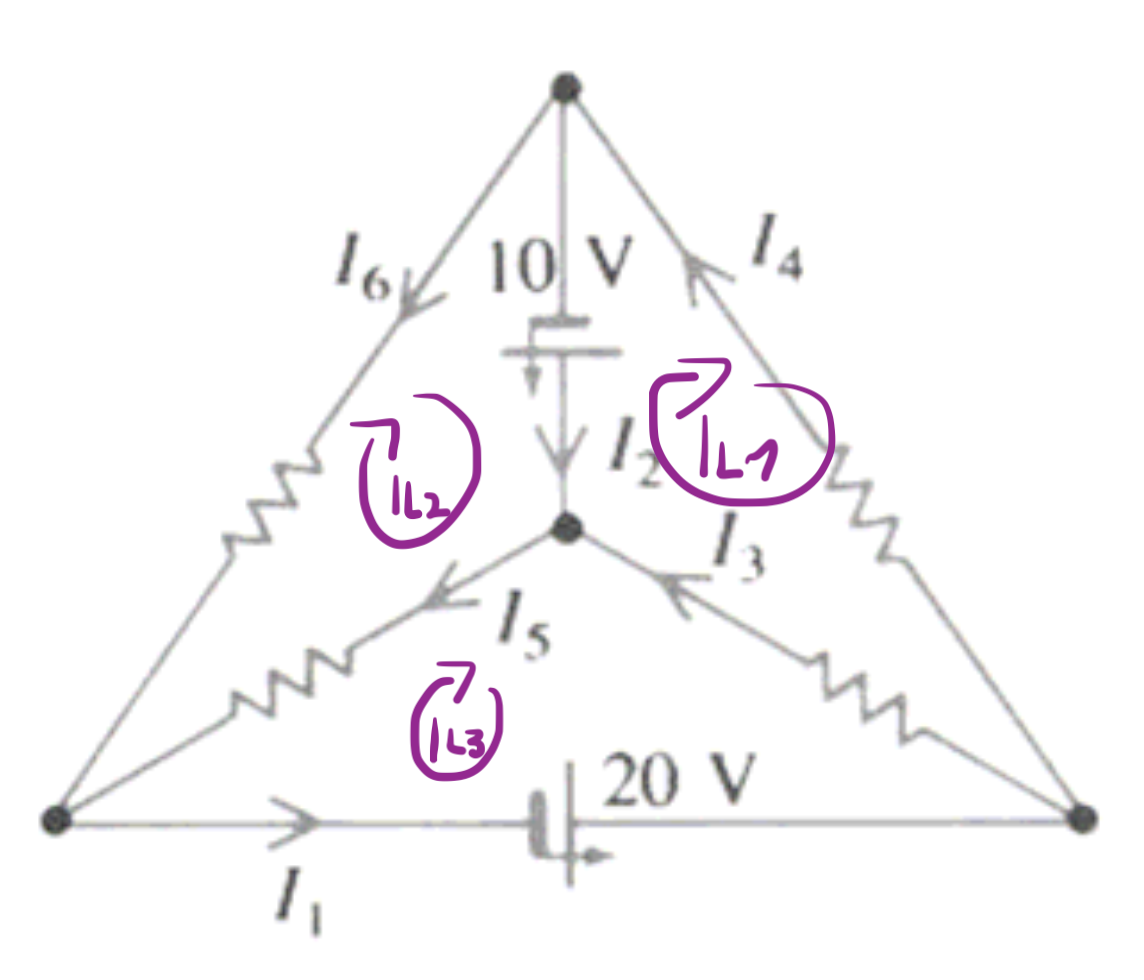
\includegraphics[width=0.5\textwidth]{images/electro.png}
    \label{fig:electro}
\end{figure}

\subsubsection*{Solution}

\begin{equation*}
    \left\{\begin{matrix}
I_{L1}(R_1 + R_2) - I_{L3}(R_2) = -E_2\\ 
I_{L2}(R_3 + R_4) - I_{L3}(R_3) = E_2\\ 
-I_{L1}(R_2) - I_{L2}(R_3) + I_{L3}(R_2 + R_3) = -E_1
\end{matrix}\right.
\end{equation*}

After substitution we have:

\begin{equation*}
    \begin{amatrix}{1}{1}
        \matr{A} & \matr{b}
    \end{amatrix} = 
    \begin{amatrix}{3}{1}
        20 & 0 & -10 & -10 \\
        0 & 20 & -10 & 10 \\
        -10 & -10 & 20 & -20
    \end{amatrix}
    \xrightarrow[magic]{}
    \begin{amatrix}{3}{1}
        1 & 0 & 0 & -1.5 \\
        0 & 1 & 0 & -0.5 \\
        0 & 0 & 1 & -2
    \end{amatrix}
\end{equation*}

\begin{equation*}
\left\{\begin{matrix}
I_1 = -I_{L3} \\
I_2 = -I_{L1} + I_{L2} \\
I_3 = I_{L1} - I_{L3} \\
I_4 = -I_{L1} \\
I_5 = I_{L2} - I_{L3} \\
I_6 = -I_{L2}
\end{matrix}\right.
\end{equation*}

\begin{equation*}
\left\{\begin{matrix}
I_1 = 2 \\
I_2 = 1 \\
I_3 = 0.5 \\
I_4 = 1.5 \\
I_5 = 1.5 \\
I_6 = 0.5
\end{matrix}\right.
\end{equation*}


% \section{Algorithms}
% \subsection{Algorithm 1 -- Gaussian elimination}\label{algorithm:1}
% \lstinputlisting[style=Matlab-editor]{algorithms/Alg1.m}
% \subsection{Algorithm 2 -- Gaussian  elimination  with  Complete  Pivoting}\label{algorithm:2}
% \lstinputlisting[style=Matlab-editor]{algorithms/Alg2.m}
% \subsection{Algorithm 3 -- Forward Substitution}\label{algorithm:3}
% \lstinputlisting[style=Matlab-editor]{algorithms/Alg3.m}
% \subsection{Algorithm 4 -- Back Substitution}\label{algorithm:4}
% \lstinputlisting[style=Matlab-editor]{algorithms/Alg4.m}
% \subsection{Algorithm 5 -- The Gauss-Jordan elimination algorithm}\label{algorithm:5}
% \lstinputlisting[style=Matlab-editor]{algorithms/Alg5.m}
% \subsection{Algorithm 6 -- The RREF algorithm}\label{algorithm:6}
% \lstinputlisting[style=Matlab-editor]{algorithms/Alg6_RREF.m}
% \subsection{Algorithm 7 -- The LU  factorization without pivoting}\label{algorithm:7}
% \lstinputlisting[style=Matlab-editor]{algorithms/Alg7.m}
% \subsection{Algorithm 8 -- The LU  factorization with partial pivoting}\label{algorithm:8}
% \lstinputlisting[style=Matlab-editor]{algorithms/Alg8.m}
% % \subsection{Algorithm 9 -- A family of the Cholesky  factorization  algorithms}\label{algorithm:9}
% % \lstinputlisting[style=Matlab-editor]{algorithms/Alg9.m}
% \stepcounter{subsection}
% \subsection{Algorithm 10 -- The Cholesky factorization}\label{algorithm:10}
% \lstinputlisting[style=Matlab-editor]{algorithms/Alg10.m}
% \subsection{Algorithm 11 -- The  QR  algorithm  by  the  Householder  transformation}\label{algorithm:11}
% \lstinputlisting[style=Matlab-editor]{algorithms/Alg11.m}
% \subsection{Algorithm 12 -- The QR algorithm by the Givens rotations}\label{algorithm:12}
% \lstinputlisting[style=Matlab-editor]{algorithms/Alg12.m}
% \subsection{Algorithm 13 -- The QR algorithm by the Gram-Schmidt orthogonalization}\label{algorithm:13}
% \lstinputlisting[style=Matlab-editor]{algorithms/Alg13.m}

%%%%%%%%%%%%%%%%%%%
%% BIBLIOGRAPHY %%%
%%%%%%%%%%%%%%%%%%%

\clearpage

\nocite{Zdunek, GoluVanl96}
\bibliographystyle{alpha}
\bibliography{bibliography}

\end{document}